\section{Avaliação de Desempenho: Nativo vs. Virtualizado}

Com o intuito de avaliar a propriedade de eficiência de virtualização, foram realizados testes experimentais para mensurar o impacto
do hipervisor no desempenho das aplicações executadas sobre as \glspl{vm}. Para essa avaliação, foram utilizados 10 \textit{benchmarks} da suíte \textit{MiBench}~\cite{mibench}:

\begin{itemize}
    \item \textbf{\textit{Basicmath}:} realiza cálculos matemáticos básicos, avaliando o desempenho em processamento numérico e operações aritméticas;
    \item \textbf{\textit{Dijkstra}:} aplica o algoritmo de Dijkstra para calcular os caminhos mais curtos em um grafo, simulando cargas de trabalho de roteamento de redes e algoritmos de navegação;
        \item \textbf{\textit{Qsort}:} executa a ordenação de um arranjo por meio do algoritmo \textit{QuickSort};
    \item \textbf{\textit{SHA}:} executa o \textit{Secure Hash Algorithm}, mensurando o desempenho do sistema sob processamento intensivo de operações bit a bit;
    \item \textbf{\textit{Susan}:} realiza o processamento de imagens para detecção de bordas, cantos e filtragem de ruído, representando tarefas de visão computacional e manipulação de matrizes de pixels.
\end{itemize}


\begin{figure}[H]
\centering
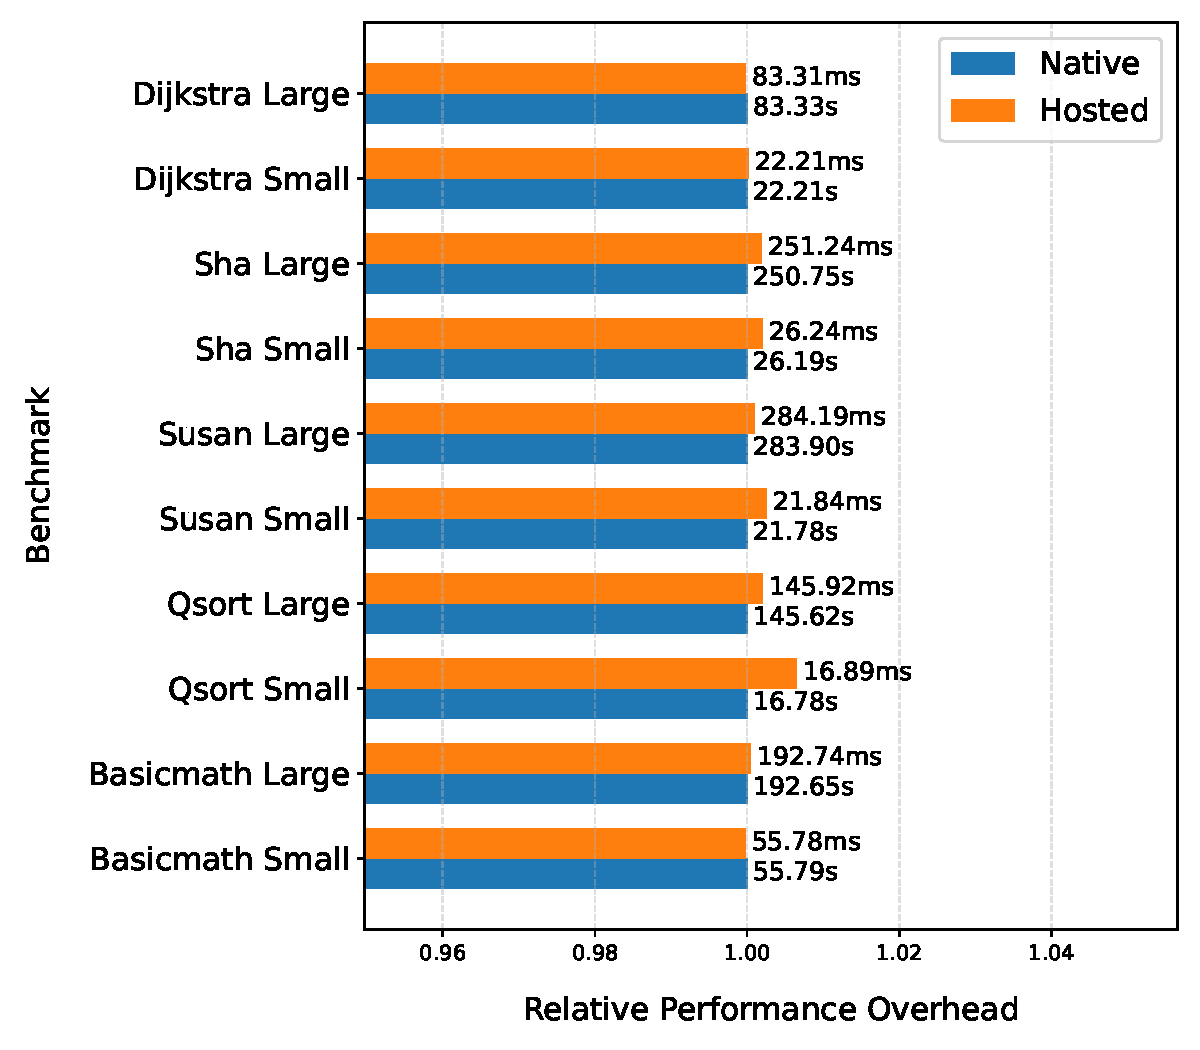
\includegraphics[width=0.7\textwidth]{images/NativeHostedBenchmarks.pdf}
\caption{Avaliação Experimental do \textit{Overhead} de Virtualização com a Suíte MiBench.}\label{fig:native-x-hosted-benchmarks}
\end{figure}

As variações \textit{Large} e \textit{Small} da Figura~\ref{fig:native-x-hosted-benchmarks} diferem estritamente no volume dos dados de entrada fornecidos a cada algoritmo,
permitindo analisar o comportamento do hipervisor tanto sob condições de estresse prolongado quanto em execuções de curta duração.

Os resultados experimentais confirmam a eficiência do hipervisor, apresentando um \textit{overhead} máximo inferior a 2\% em todos os testes.
Tal fato, evidencia que a camada de virtualização mantém o desempenho das \glspl{vm} próximo ao da execução nativa.
